The organization of the architecture is described in Figure \ref{fig:gen}.

\begin{figure}[!h]
\centering
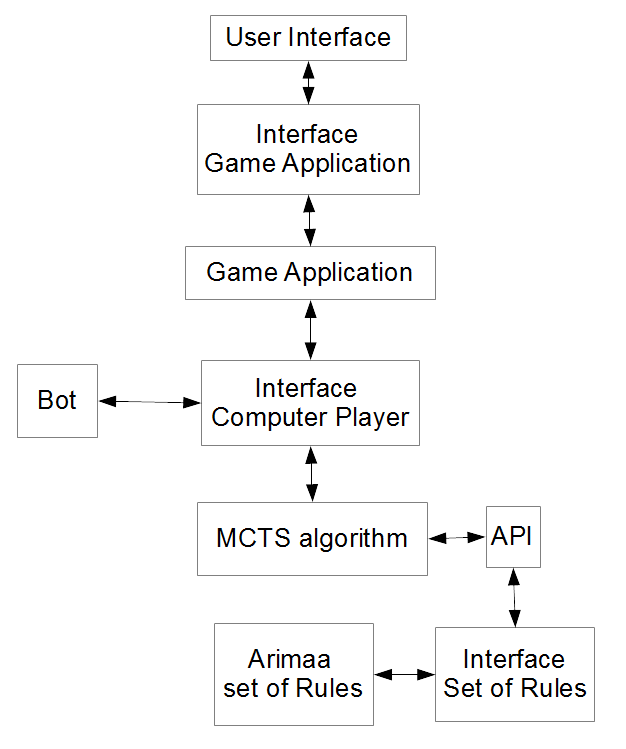
\includegraphics[width=0.8\textwidth]{2General_Architecture/2.1.2GeneralView/gen.png}
\caption{General view of the architecture}
\label{fig:gen}
\end{figure}

The user will interact with the Interface, which will communicate with the Game Application, where all data for the game will be store. Then, it will communicate with an Interface which will handle the communications between the Game application and the computer player. 

In our case, the computer player will be played by the MCTS algorithm, communicating to the Arimaa set of rules via the API and an interface for the set of Rules.  If another algorithm is willing to be tested, it will be added.  If another algorithm is willing to be tested, it will be added.

Interfaces are very important because they make it possible for others to use our project for others games than Arimaa without rebuilding everything. They would have just to implement the Interface with their proper game, game rules.

Furthermore, if the time permits it, the management of computers bots\footnote{For instance of the site \textit{Arimaa.com}} will be added. The only problem here is the computers bots are not similar to each others, thus it will take time to implement a class which will be able to communicate with both the computer bot and the interface.

The input of our software will be the action of the users, his mouse clics, moves with keyboard. The Output will only be the display of the screen, after a move of the opponent in 1VSComputer or nothing in 1VS1.